% !TEX root = main.tex

%\paragraph{PCA Assumption}
\label{sec:experimentsPCA}

%\comment{R3}{I would like to understand sooner that 4.3 is a discarded and useless digression and I would appreciate a deeper discussion of Section 4.4,  possibly with examples (note that 4.4 and 4.4.2 have the same title, which is not elegant)}

% \comment{Chris}{Removed PosOnly evaluation function, merged PCA assumption-PCA confidence. Discussed by example of table 1. Removed the FUN-property stuff}

% Fabian: Thanks! I made my pass.


The support of a rule quantifies the number of known correct predictions of the rule.
However, it does not take into account the false predictions of the rule.
Following \cite{amie}, we will now describe measures that judge the \emph{quality} of a rule.
We first describe the challenges in defining such a measure in our setting
and discuss the most common way to measure the rule quality, which we call the standard confidence.
Then, we introduce our own measure: the confidence under the assumption of partial completeness.



% The support of a rule quantifies the number of known correct predictions of the rule. However, it does not measure the false predictions of the rule.
% We will now describe measures that judge the rule \emph{quality}.
% We first describe the challenges in defining such a measure in our setting %of our setting w.r.t. designing a good measure for judging the quality of a rule,
% and discuss existing measures: the standard confidence and the Positive-Only Learning score.
% Then, we introduce our own measure: the confidence under the assumption of partial completeness.
% We also discuss the practical applicability of this assumption.

\subsection{Challenges}
Let us consider a given Horn rule $\vec{B} \Rightarrow r(x,y)$. Let us look at all facts with relation $r$ (Figure \ref{fig:prediction}).
We distinguish 4 types of facts: True facts that are known to the KB (KBtrue), true facts that are unknown to the KB (NEWtrue),
facts that are known to be false in the KB (KBfalse), and facts that are false but unknown to the KB (NEWfalse).
The rule will make certain predictions about relation $r$ (blue circle). These predictions can be known to be true (A), known to be false (C), or unknown (B and D).
When they are unknown to the KB, they can still be true (B) or false (D) with respect to the real world.\\

%\ffigure{Figure}{model}{\label{fig:prediction}Prediction under Incompleteness}{% This is the TIKZ version of the file
%     model.svg
% generated by PowerLine, the free SVG editor with Latex support

% To include this picture in LaTex, write the following in its preamble:
%  \usepackage{tikz}
%  \usepackage{graphicx}
%  \usepackage{hyperref}
% Then write '% !TEX root = main.tex

\www{
\paragraph{Model} We follow the description of the mining model from \cite{amie}.
Let us consider a given Horn rule $\vec{B} \Rightarrow r(x,y)$. Let us look at all facts with relation $r$ (Figure \ref{model}). 
We distinguish 4 types of facts: True facts that are known to the KB (KBtrue), true facts that are unknown to the KB (NEWtrue), 
facts that are known to be false in the KB (KBfalse), and facts that are false but unknown to the KB (NEWfalse). 
The rule will make certain predictions (blue circle). These predictions can be known to be true (A), known to be false (C), or unknown (B and D). 
When they are unknown to the KB, they can still be true (B) or false (D) with respect to the real world.\\

\ffigure{Figure}{model}{\label{fig:prediction}Prediction under Incompleteness}{% This is the TIKZ version of the file
%     model.svg
% generated by PowerLine, the free SVG editor with Latex support

% To include this picture in LaTex, write the following in its preamble:
%  \usepackage{tikz}
%  \usepackage{graphicx}
%  \usepackage{hyperref}
% Then write '\input{model.tikz}' where the picture shall appear in the LaTex document.

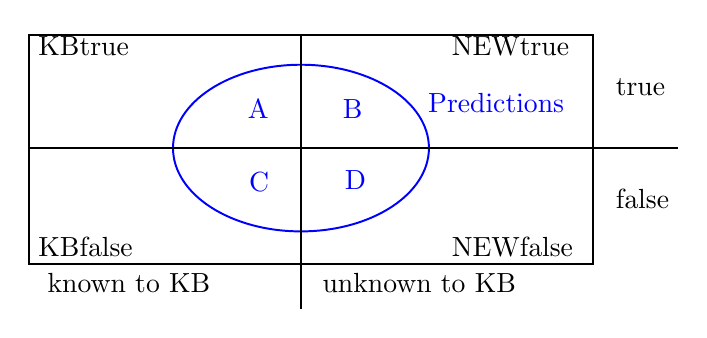
\begin{tikzpicture}

% Fabian: Keep figure in two colors.
% Even if printed in black and white, it's still clear enough

  \path[draw=blue, line width=0.7086614168764338] (3.708333, -1.458333) ellipse (1.625000 and 1.058333);
  \node[above, right, color=blue, font=] at (5.2000, -0.88333) {Predictions};
  \node[above, right, color=blue, font=] at (2.908333, -0.958333) {A};
  \node[above, right, color=blue, font=] at (4.116667, -0.966667) {B};
  \node[above, right, color=blue, font=] at (2.925000, -1.891667) {C};
  \node[above, right, color=blue, font=] at (4.141667, -1.866667) {D};
  \node[above, right, color=black, font=] at (0.250000, -0.166667) {KBtrue};
  \node[above, right, color=black, font=] at (0.250000, -2.708333) {KBfalse};
  \node[above, right, color=black, font=] at (5.500000, -0.166667) {NEWtrue};
  \node[above, right, color=black, font=] at (5.500000, -2.708333) {NEWfalse};
  \node[above, right, color=black, font=] at (7.583333, -0.683333) {true};
  \node[above, right, color=black, font=] at (7.583333, -2.100000) {false};
  \node[above, right, color=black, font=] at (0.366667, -3.166667) {known to KB};
  \node[above, right, color=black, font=] at (3.858333, -3.166667) {unknown to KB};
  \path[draw=black, line width=0.7086614168764338] (0.250000, -0.016667) rectangle (7.416667, -2.933333);
  \draw[draw=black, line width=0.7086614168764338] (0.250000, -1.458333) -- (8.500000, -1.458333);
  \draw[draw=black, line width=0.7086614168764338] (3.708333, -0.025000) -- (3.708333, -3.500000);
\end{tikzpicture}
}

}

\www{
\paragraph{Goal} 
Our goal is to find rules that make true predictions that go beyond the current KB. 
In the figure, we wish to maximize the area B, and to minimize the area D. 
There are two obvious challenges in this context: First, the areas NEWtrue and NEWfalse are unknown. 
So if we wish to maximize B at the expense of D, we are operating in an area outside our KB. 
We would want to use the areas KBtrue and KBfalse to estimate the unknown area. 
This, however, leads to the second challenge: Semantic KBs do not contain negative evidence. 
Thus, the area KBfalse is empty. In the following, we discuss different measures that address these challenges.
}

% \www{
% \paragraph{Support} 
% The \emph{support} of a rule quantifies the number of correct predictions, i.e., the size of A. There are several ways to define the support: It can be the number of instantiations of the rule that appear in the KB. This is what our analogy to association rule mining \cite{AgrImiSwa93} suggests (Section \ref{sec:preliminaries}). This measure, however, is not monotonic if we add atoms to the body. Consider, for example, the rule
% \indented{
%   \emph{marriedTo(}$x,y) \Rightarrow$ \emph{marriedTo(}$y,x$)
% }
% If we add \emph{hasGender($x$,male)} to the body, the number of instantiations that are in the KB decreases. If we add an atom with a fresh variable, e.g., \emph{hasFriend($x$,$z$)}, to the body, the number of instantiations increases for every friend of $x$. This is true even if we add another atom with $z$ to make the rule closed.\
% Alternatively, we can count the number of facts in one particular body atom.
% This definition, however, depends on the choice of the body atom, so that the same rule can have different supports. We can also count the number of facts of the head atom.
% This measure decreases monotonically if more body atoms are added 
% and avoids equivalent rules with different support values. With this in mind, we define the support of a rule as the number of distinct pairs of subjects and objects in the head of all instantiations that appear in the KB:
% \[supp(\vec{B} \Rightarrow r(x,y)) := \#(x,y): \exists z_1,...,z_m: \vec{B} \wedge r(x,y)\]
% where $z_1,...,z_m$ are the variables of the rule apart from $x$ and $y$.
% }

\www{
\paragraph{Support} 
The \emph{support} of a rule quantifies the number of correct predictions, i.e., the size of A. 
There are several ways to define the support: It can be the number of instantiations of the rule that appear in the KB. 
%This is what our analogy to association rule mining \cite{AgrImiSwa93} suggests (Section \ref{sec:preliminaries}). \comment{Katja}{Remove this sentence if the section about association rule mining is removed permanently.}
This measure, however, is not monotonic if we add atoms to the body. Consider, for example, the rule
\indented{
  \emph{marriedTo(}$x,y) \Rightarrow$ \emph{marriedTo(}$y,x$)
}
If we add \emph{hasGender($x$,male)} to the body, the number of instantiations that are in the KB decreases. 
If we add an atom with a fresh variable, e.g., \emph{hasFriend($x$,$z$)}, to the body, the number of instantiations increases for every friend of $x$. 
This is true even if we add another atom with $z$ to obtain a closed rule.\
Alternatively, we can count the number of facts in one particular body atom.
This definition, however, depends on the choice of the body atom, so that the same rule can have different supports. 
We can also count the number of facts of the head atom.
This measure decreases monotonically if more body atoms are added and avoids equivalent rules with different support values. 
With this in mind, we define the support of a rule as the number of distinct pairs of subjects and objects in the head of all instantiations that appear in the KB:
\[supp(\vec{B} \Rightarrow r(x,y)) := \#(x,y): \exists z_1,...,z_m: \vec{B} \wedge r(x,y)\]
where $z_1,...,z_m$ are the variables of the rule apart from $x$ and $y$. }
Note that the support is defined even for rules that are not closed.


% \www{
% \paragraph{Head Coverage} %\comment{check again}
% % Support is an absolute number. This means that a user who thresholds on support has to know the absolute size of the KB to give meaningful values. 
% % To avoid this, we also need to define a proportional version of support, the \emph{head coverage}. It is the proportion of pairs from the head relation that are covered by the predictions of the rule:
% % \[hc(\vec{B} \Rightarrow r(x,y)) := \frac{supp(\vec{B} \Rightarrow r(x,y))}{\#(x,y) : r(x,y)}\]
% Support is an absolute number. This means that a user who thresholds on support has to know the absolute size of the KB to give meaningful values. 
% To avoid this, we also define a proportional version of support. A naive way would be to use the absolute number of support, as defined in the previous paragraph, over the size of the KB. 
% In this case, however, relations that do not have many facts (either because of the incompleteness of the KB or because of their nature), will not be considered in the head of rules,
% i.e. we will not learn rules predicting such relations. Therefore, we propose to use the notion of \emph{head coverage}. 
% This is the proportion of pairs from the head relation that are covered by the predictions of the rule
% % Head coverage is the proportion of pairs from the head relation that are covered by the predictions of the rule:
% \[hc(\vec{B} \Rightarrow r(x,y)) := \frac{supp(\vec{B} \Rightarrow r(x,y))}{\#(x',y') : r(x',y')}\]
% }


\www{
\paragraph{Head Coverage}
Support is an absolute number. This means that a user defining thresholds on support has to know the absolute size of the KB to give meaningful values. 
To avoid this, we propose a proportional version of support. A naive way would be to use the absolute number of support, as defined in the previous paragraph, over the size of the KB. 
In this case, however, relations that do not have many facts (either because of the incompleteness of the KB or because of their nature) will not be considered in the head of the rules,
i.e., we will not learn rules predicting such relations. Therefore, we propose to use the notion of \emph{head coverage}:
\[hc(\vec{B} \Rightarrow r(x,y)) := \frac{supp(\vec{B} \Rightarrow r(x,y))}{size(r)}\]
}

with $size(r) := \#(x',y') : r(x',y')$ denoting the number of facts in relation $r$.

Head coverage quantifies the percentage of the known true facts that are implied %(for the case of closed rules) %or can possibly be implied (for the case of not yet closed rules)
% Fabian: I think that this description is sufficient. The mroe precise one risks confusing readers.
by the rule.
Head coverage can be a measure of statistical significance for any measure used to evaluate the quality of a rule. 
\comment{Fabian}{I am not sure about this. Could you explain? If it is not crucial here, I would omit it at this position.}



\www{
\paragraph{Negative Examples} 
The central challenge of our setting is to provide counter-examples for the rule mining. 
These can take the role of KBfalse, so that we can estimate the areas NEWtrue and NEWfalse. 
There are several approaches to this problem: The standard confidence, the standard positive-only learning evaluation score of ILP, and the partial completeness assumption that we propose. 
}
We will now present these approaches in detail.

% \www{
% \paragraph{Standard Confidence} 
% The standard confidence measure takes all facts that are not in the KB (i.e., NEWtrue and NEWfalse) as negative evidence. 
% Thus, the standard confidence of a rule is the ratio of its predictions that are in the KB, i.e., the share of A in the set of predictions:
% \[conf(\vec{B} \Rightarrow r(x,y)) := \frac{supp(\vec{B} \Rightarrow r(x,y))}{\#(x,y): \exists z_1,...,z_m: \vec{B}}\]
% %\[conf(\vec{B} \Rightarrow r(x,y)) := \frac{supp(\vec{B} \Rightarrow r(x,y))}{supp(\vec{B})}\]
% The standard confidence is blind to the distinction between ``false'' and ``unknown''. Thus, it implements a closed world setting. It mainly describes the known data and penalizes rules that make a large number of predictions in the unknown region. We, in contrast, aim to maximize the number of true predictions that go beyond the current knowledge. We do not want to describe data, but to predict data.
% }



\www{
\paragraph{Standard Confidence} 
The standard confidence measure takes all facts that are not in the KB (i.e., NEWtrue and NEWfalse) as negative evidence. 
Thus, the standard confidence of a rule is the ratio of its predictions that are in the KB, i.e., the share of A (KBtrue) in the set of predictions:
%\[conf(\vec{B} \Rightarrow r(x,y)) := \frac{supp(\vec{B} \Rightarrow r(x,y))}{\#(x,y): \exists z_1,...,z_m: \vec{B}}\]
}

%\comment{Katja}{I prefer the second one.}
\[conf(\vec{B} \Rightarrow r(x,y)) := \frac{\#(x,y): \exists z_1,...,z_m: \vec{B} \wedge r(x,y)}{\#(x,y): \exists z_1,...,z_m: \vec{B}}\]
%\[conf(\vec{B} \Rightarrow r(x,y)) := \frac{supp(\vec{B} \Rightarrow r(x,y))}{supp(\vec{B})}\]

Standard confidence is the measure traditionally used in association rule mining and market basket analysis, where a Closed World Assumption (CWA) is made: 
if there is no evidence in any of the transactions of the database that a user bought a specific product, then this user did not buy the product.
Although natural for the market basket analysis scenario, standard confidence fails to distinguish between ``false'' and ``unknown'' facts, 
which makes it inappropriate for a scenario with Open World semantics, like ours. Moreover, we also persue a different goal than market basket analysis:
we aim to maximize the number of true predictions that go beyond the current knowledge, whereas market basket analysis usually tries to mine rules that can describe data that is already known. 






\www{
\paragraph{Positive-Only Learning} 
For cases where the KB does not contain negative examples, Muggleton has developed a \emph{positive-only learning evaluation score} for ILP \cite{Muggleton:1996:LPD:647996.742465},\cite{usir1753}. 
It takes random facts as negative evidence:
\[
 Score = log(P)-log\frac{R+1}{Rsize+2}-\frac{L}{P}
\]
Here, $P$ is the number of known true facts covered (KBtree, or A resp., in Figure~\ref{fig:prediction}), $R$ is the number of randoms covered, $Rsize$ is the total number of randoms and $L$ is the number of atoms in the hypotheses. 
The intuition is that a good rule should cover many positive examples, and few or no randomly generated examples. This ensures  
that the rule is not overly general. Furthermore, the rule should use as few atoms as possible, and thus achieve a high compression. This measure is implemented (among others) in the ALEPH system.
}


% \www{
% \paragraph{Partial Completeness} 
% We propose to generate negative evidence by the \emph{partial completeness assumption} (PCA).
% This is the assumption that if $r(x,y) \in$ \emph{KBtrue} for some $x,y$, then
% \[\forall y': r(x,y') \in \mbox{\emph{KBtrue}} \cup \mbox{\emph{NEWtrue}} \Rightarrow r(x,y') \in \mbox{\emph{KBtrue}}\] 
% In other words, we assume that if the database knows some $r$-attribute of $x$, then it knows all $r$-attributes of $x$. This assumption is certainly true for functional relations $r$, 
% such as birth dates, capitals, etc. Thanks to the FUN-Property (see Section \ref{sec:model}), it is also true for inverse-functional relations, such as \emph{owns}, \emph{created}, etc. 
% The assumption is also true in the vast majority of cases for relations that are not functional, but that have a high functionality. 
% Even for other relations, the PCA is still reasonable for knowledge bases that have been extracted from a single source (such as DBpedia and YAGO). 
% These usually contain either all $r$-values or none for a given entity.
% }


\paragraph{Partial Completeness} 
We propose to generate negative evidence by means of the \emph{partial completeness assumption} (PCA).
This is the assumption that if $r(x,y) \in$ \emph{KBtrue} for some $x,y$,
%and $x$ is the input variable, 
% Fabian: we already said that all relations are more functional than inverse functional
then
\[\forall y': r(x,y') \in \mbox{\emph{KBtrue}} \cup \mbox{\emph{NEWtrue}} \Rightarrow r(x,y') \in \mbox{\emph{KBtrue}}\] 
%In other words, we assume that if the database knows some $r$-attribute of $x$, then it knows all $r$-attributes of $x$. 
%In other words, we assume that if the database knows some entity for the output variable $y$ for a given relation $r$ and entity of the input variable $x$, 
%then it knows all possible entities for the  output variable $y$ for these $r$ and $x$.
%\comment{Katja}{The term ``$r$-attribute of $x$'' is not intuitive for the reader as it has not been formally introduced, and the term attribute occurs only here. I suggest to replace it.}
% Fabian: I gave it another try, without the input and output:
In other words, we assume that if we know one $y$ for a given $x$, then we know all $y$ for that $x$.

This assumption is certainly true for functional relations $r$, such as \emph{birthdates} and \emph{capitals}.
Thanks to the FUN-property, the assumption is also true for inverse-functional relations, such as \emph{owns} and \emph{created}.
%, with the difference that in this case $x$ is the output variable and $y$ the input variable.
%, with the difference that in this case we assume that we know all $r$-attributes of $y$ (since $y$ is the input variable in this case).
The assumption is also true in the vast majority of cases for relations that are not functional, but that have a high functionality. 
Even for other relations, the PCA is still reasonable for knowledge bases that have been extracted from a single source (such as DBpedia and YAGO), as we shall see. 
%These usually contain either all $r$-values or none for a given entity. \comment{Katja}{Likewise, the term ``$r$-values'' is not introduced.}
We present an experimental evaluation of the PCA in Section~\ref{sec:experimentsPCA}.

% \www{
% \paragraph{PCA Confidence} 
% Under the PCA, we normalize the confidence not by the entire set of facts, but by the set of facts of which we know that they are true, together with the facts of which we assume that they are false. If the head atom of the rule is $r(x,y)$, then this set is just the set of facts $\{ r(x,y') : r(x,y') \in \mathcal{K}\}$. Thanks to the FUN-Property, the PCA is always applied to the first argument of the head atom:
% %\[pcaconf(\vec{B} \Rightarrow r(x,y)) := \frac{\#(x,y): \exists z_1,...,z_m: \vec{B} \wedge r(x,y)}{\#(x,y): \exists z_1,...,z_m,y': \vec{B} \wedge r(x,y')}\]
% \[pcaconf(\vec{B} \Rightarrow r(x,y)) := \frac{supp(\vec{B} \Rightarrow r(x,y))}{\#(x,y): \exists z_1,...,z_m,y': \vec{B} \wedge r(x,y')}\]
% We show in our experiments that the PCA confidence identifies much more productive rules than the other measures.
% }



\paragraph{PCA Confidence} 
\label{pcaConf}
Under the PCA, the denominator of the confidence will not be the size of the entire set of facts that the body of the rule produces, 
but the number of facts that we know to be true together with the facts that we assume to be false. 
\comment{Fabian}{Important fix here: Christina found that the denominator should count $\#(x,y)$, and not $\#(x,y')$.}

% If the head atom of the rule is $r(x,y)$, then this set is just the set of facts $\{ r(x,y') : r(x,y') \in \mathcal{K}\}$. 
% The PCA confidence for a rule with $x$ as the input variable is defined as:
% \[
% \small \hspace*{-1ex}
% conf_{PCA}(\vec{B} \Rightarrow r(x,y)) := \frac{supp(\vec{B} \Rightarrow r(x,y))}{\#(x,y): \exists z_1,...,z_m,y': \vec{B} \wedge r(x,y')}
% \]
% \comment{Katja}{If we replace the formula for the standard confidence, we should use the same notation here:
\[
\small \hspace*{-2ex}
conf_{PCA}(\vec{B} \Rightarrow r(x,y)) := \frac{\#(x,y): \exists z_1,...,z_m: \vec{B} \wedge r(x,y)}{\#(x,y): \exists z_1,...,z_m,y': \vec{B} \wedge r(x,y')}
\]
%}
This confidence normalizes the support by the number of pairs $(x,y)$ for which there exists a $y'$ with $r(x,y')$, i.e., for which we assume that the KB knows all such $y'$.
\comment{Chris}{Think about if you want to include the following one.} 
\comment{Katja}{I suggest to remove it because we will have a detailed discussion in the experiments and do not need it already here.}
The PCA confidence can be seen as a process in which we first take a biased sample of the body (those facts containing entities for the $x$ variable that appear also in the head)
and then calculate the standard confidence over this sample. 
The fact that our sample is biased implies that PCA confidence might not be a good estimator of the actual predictive power of the rule (precision).
However, our experiments show that overall PCA confidence identifies much more productive rules than the other measures and it also correlates with precision better than the standard confidence.' where the picture shall appear in the LaTex document.

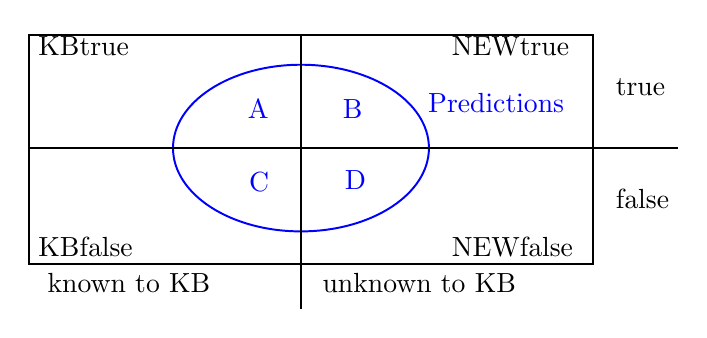
\begin{tikzpicture}

% Fabian: Keep figure in two colors.
% Even if printed in black and white, it's still clear enough

  \path[draw=blue, line width=0.7086614168764338] (3.708333, -1.458333) ellipse (1.625000 and 1.058333);
  \node[above, right, color=blue, font=] at (5.2000, -0.88333) {Predictions};
  \node[above, right, color=blue, font=] at (2.908333, -0.958333) {A};
  \node[above, right, color=blue, font=] at (4.116667, -0.966667) {B};
  \node[above, right, color=blue, font=] at (2.925000, -1.891667) {C};
  \node[above, right, color=blue, font=] at (4.141667, -1.866667) {D};
  \node[above, right, color=black, font=] at (0.250000, -0.166667) {KBtrue};
  \node[above, right, color=black, font=] at (0.250000, -2.708333) {KBfalse};
  \node[above, right, color=black, font=] at (5.500000, -0.166667) {NEWtrue};
  \node[above, right, color=black, font=] at (5.500000, -2.708333) {NEWfalse};
  \node[above, right, color=black, font=] at (7.583333, -0.683333) {true};
  \node[above, right, color=black, font=] at (7.583333, -2.100000) {false};
  \node[above, right, color=black, font=] at (0.366667, -3.166667) {known to KB};
  \node[above, right, color=black, font=] at (3.858333, -3.166667) {unknown to KB};
  \path[draw=black, line width=0.7086614168764338] (0.250000, -0.016667) rectangle (7.416667, -2.933333);
  \draw[draw=black, line width=0.7086614168764338] (0.250000, -1.458333) -- (8.500000, -1.458333);
  \draw[draw=black, line width=0.7086614168764338] (3.708333, -0.025000) -- (3.708333, -3.500000);
\end{tikzpicture}
}
\begin{figure}[h]
\caption{Prediction under Incompleteness}
% This is the TIKZ version of the file
%     model.svg
% generated by PowerLine, the free SVG editor with Latex support

% To include this picture in LaTex, write the following in its preamble:
%  \usepackage{tikz}
%  \usepackage{graphicx}
%  \usepackage{hyperref}
% Then write '% !TEX root = main.tex

\www{
\paragraph{Model} We follow the description of the mining model from \cite{amie}.
Let us consider a given Horn rule $\vec{B} \Rightarrow r(x,y)$. Let us look at all facts with relation $r$ (Figure \ref{model}). 
We distinguish 4 types of facts: True facts that are known to the KB (KBtrue), true facts that are unknown to the KB (NEWtrue), 
facts that are known to be false in the KB (KBfalse), and facts that are false but unknown to the KB (NEWfalse). 
The rule will make certain predictions (blue circle). These predictions can be known to be true (A), known to be false (C), or unknown (B and D). 
When they are unknown to the KB, they can still be true (B) or false (D) with respect to the real world.\\

\ffigure{Figure}{model}{\label{fig:prediction}Prediction under Incompleteness}{% This is the TIKZ version of the file
%     model.svg
% generated by PowerLine, the free SVG editor with Latex support

% To include this picture in LaTex, write the following in its preamble:
%  \usepackage{tikz}
%  \usepackage{graphicx}
%  \usepackage{hyperref}
% Then write '\input{model.tikz}' where the picture shall appear in the LaTex document.

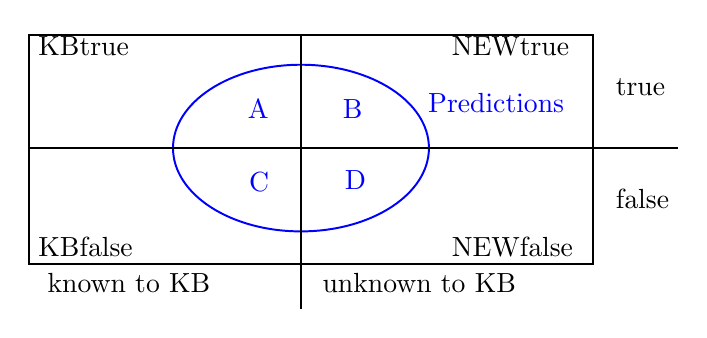
\begin{tikzpicture}

% Fabian: Keep figure in two colors.
% Even if printed in black and white, it's still clear enough

  \path[draw=blue, line width=0.7086614168764338] (3.708333, -1.458333) ellipse (1.625000 and 1.058333);
  \node[above, right, color=blue, font=] at (5.2000, -0.88333) {Predictions};
  \node[above, right, color=blue, font=] at (2.908333, -0.958333) {A};
  \node[above, right, color=blue, font=] at (4.116667, -0.966667) {B};
  \node[above, right, color=blue, font=] at (2.925000, -1.891667) {C};
  \node[above, right, color=blue, font=] at (4.141667, -1.866667) {D};
  \node[above, right, color=black, font=] at (0.250000, -0.166667) {KBtrue};
  \node[above, right, color=black, font=] at (0.250000, -2.708333) {KBfalse};
  \node[above, right, color=black, font=] at (5.500000, -0.166667) {NEWtrue};
  \node[above, right, color=black, font=] at (5.500000, -2.708333) {NEWfalse};
  \node[above, right, color=black, font=] at (7.583333, -0.683333) {true};
  \node[above, right, color=black, font=] at (7.583333, -2.100000) {false};
  \node[above, right, color=black, font=] at (0.366667, -3.166667) {known to KB};
  \node[above, right, color=black, font=] at (3.858333, -3.166667) {unknown to KB};
  \path[draw=black, line width=0.7086614168764338] (0.250000, -0.016667) rectangle (7.416667, -2.933333);
  \draw[draw=black, line width=0.7086614168764338] (0.250000, -1.458333) -- (8.500000, -1.458333);
  \draw[draw=black, line width=0.7086614168764338] (3.708333, -0.025000) -- (3.708333, -3.500000);
\end{tikzpicture}
}

}

\www{
\paragraph{Goal} 
Our goal is to find rules that make true predictions that go beyond the current KB. 
In the figure, we wish to maximize the area B, and to minimize the area D. 
There are two obvious challenges in this context: First, the areas NEWtrue and NEWfalse are unknown. 
So if we wish to maximize B at the expense of D, we are operating in an area outside our KB. 
We would want to use the areas KBtrue and KBfalse to estimate the unknown area. 
This, however, leads to the second challenge: Semantic KBs do not contain negative evidence. 
Thus, the area KBfalse is empty. In the following, we discuss different measures that address these challenges.
}

% \www{
% \paragraph{Support} 
% The \emph{support} of a rule quantifies the number of correct predictions, i.e., the size of A. There are several ways to define the support: It can be the number of instantiations of the rule that appear in the KB. This is what our analogy to association rule mining \cite{AgrImiSwa93} suggests (Section \ref{sec:preliminaries}). This measure, however, is not monotonic if we add atoms to the body. Consider, for example, the rule
% \indented{
%   \emph{marriedTo(}$x,y) \Rightarrow$ \emph{marriedTo(}$y,x$)
% }
% If we add \emph{hasGender($x$,male)} to the body, the number of instantiations that are in the KB decreases. If we add an atom with a fresh variable, e.g., \emph{hasFriend($x$,$z$)}, to the body, the number of instantiations increases for every friend of $x$. This is true even if we add another atom with $z$ to make the rule closed.\
% Alternatively, we can count the number of facts in one particular body atom.
% This definition, however, depends on the choice of the body atom, so that the same rule can have different supports. We can also count the number of facts of the head atom.
% This measure decreases monotonically if more body atoms are added 
% and avoids equivalent rules with different support values. With this in mind, we define the support of a rule as the number of distinct pairs of subjects and objects in the head of all instantiations that appear in the KB:
% \[supp(\vec{B} \Rightarrow r(x,y)) := \#(x,y): \exists z_1,...,z_m: \vec{B} \wedge r(x,y)\]
% where $z_1,...,z_m$ are the variables of the rule apart from $x$ and $y$.
% }

\www{
\paragraph{Support} 
The \emph{support} of a rule quantifies the number of correct predictions, i.e., the size of A. 
There are several ways to define the support: It can be the number of instantiations of the rule that appear in the KB. 
%This is what our analogy to association rule mining \cite{AgrImiSwa93} suggests (Section \ref{sec:preliminaries}). \comment{Katja}{Remove this sentence if the section about association rule mining is removed permanently.}
This measure, however, is not monotonic if we add atoms to the body. Consider, for example, the rule
\indented{
  \emph{marriedTo(}$x,y) \Rightarrow$ \emph{marriedTo(}$y,x$)
}
If we add \emph{hasGender($x$,male)} to the body, the number of instantiations that are in the KB decreases. 
If we add an atom with a fresh variable, e.g., \emph{hasFriend($x$,$z$)}, to the body, the number of instantiations increases for every friend of $x$. 
This is true even if we add another atom with $z$ to obtain a closed rule.\
Alternatively, we can count the number of facts in one particular body atom.
This definition, however, depends on the choice of the body atom, so that the same rule can have different supports. 
We can also count the number of facts of the head atom.
This measure decreases monotonically if more body atoms are added and avoids equivalent rules with different support values. 
With this in mind, we define the support of a rule as the number of distinct pairs of subjects and objects in the head of all instantiations that appear in the KB:
\[supp(\vec{B} \Rightarrow r(x,y)) := \#(x,y): \exists z_1,...,z_m: \vec{B} \wedge r(x,y)\]
where $z_1,...,z_m$ are the variables of the rule apart from $x$ and $y$. }
Note that the support is defined even for rules that are not closed.


% \www{
% \paragraph{Head Coverage} %\comment{check again}
% % Support is an absolute number. This means that a user who thresholds on support has to know the absolute size of the KB to give meaningful values. 
% % To avoid this, we also need to define a proportional version of support, the \emph{head coverage}. It is the proportion of pairs from the head relation that are covered by the predictions of the rule:
% % \[hc(\vec{B} \Rightarrow r(x,y)) := \frac{supp(\vec{B} \Rightarrow r(x,y))}{\#(x,y) : r(x,y)}\]
% Support is an absolute number. This means that a user who thresholds on support has to know the absolute size of the KB to give meaningful values. 
% To avoid this, we also define a proportional version of support. A naive way would be to use the absolute number of support, as defined in the previous paragraph, over the size of the KB. 
% In this case, however, relations that do not have many facts (either because of the incompleteness of the KB or because of their nature), will not be considered in the head of rules,
% i.e. we will not learn rules predicting such relations. Therefore, we propose to use the notion of \emph{head coverage}. 
% This is the proportion of pairs from the head relation that are covered by the predictions of the rule
% % Head coverage is the proportion of pairs from the head relation that are covered by the predictions of the rule:
% \[hc(\vec{B} \Rightarrow r(x,y)) := \frac{supp(\vec{B} \Rightarrow r(x,y))}{\#(x',y') : r(x',y')}\]
% }


\www{
\paragraph{Head Coverage}
Support is an absolute number. This means that a user defining thresholds on support has to know the absolute size of the KB to give meaningful values. 
To avoid this, we propose a proportional version of support. A naive way would be to use the absolute number of support, as defined in the previous paragraph, over the size of the KB. 
In this case, however, relations that do not have many facts (either because of the incompleteness of the KB or because of their nature) will not be considered in the head of the rules,
i.e., we will not learn rules predicting such relations. Therefore, we propose to use the notion of \emph{head coverage}:
\[hc(\vec{B} \Rightarrow r(x,y)) := \frac{supp(\vec{B} \Rightarrow r(x,y))}{size(r)}\]
}

with $size(r) := \#(x',y') : r(x',y')$ denoting the number of facts in relation $r$.

Head coverage quantifies the percentage of the known true facts that are implied %(for the case of closed rules) %or can possibly be implied (for the case of not yet closed rules)
% Fabian: I think that this description is sufficient. The mroe precise one risks confusing readers.
by the rule.
Head coverage can be a measure of statistical significance for any measure used to evaluate the quality of a rule. 
\comment{Fabian}{I am not sure about this. Could you explain? If it is not crucial here, I would omit it at this position.}



\www{
\paragraph{Negative Examples} 
The central challenge of our setting is to provide counter-examples for the rule mining. 
These can take the role of KBfalse, so that we can estimate the areas NEWtrue and NEWfalse. 
There are several approaches to this problem: The standard confidence, the standard positive-only learning evaluation score of ILP, and the partial completeness assumption that we propose. 
}
We will now present these approaches in detail.

% \www{
% \paragraph{Standard Confidence} 
% The standard confidence measure takes all facts that are not in the KB (i.e., NEWtrue and NEWfalse) as negative evidence. 
% Thus, the standard confidence of a rule is the ratio of its predictions that are in the KB, i.e., the share of A in the set of predictions:
% \[conf(\vec{B} \Rightarrow r(x,y)) := \frac{supp(\vec{B} \Rightarrow r(x,y))}{\#(x,y): \exists z_1,...,z_m: \vec{B}}\]
% %\[conf(\vec{B} \Rightarrow r(x,y)) := \frac{supp(\vec{B} \Rightarrow r(x,y))}{supp(\vec{B})}\]
% The standard confidence is blind to the distinction between ``false'' and ``unknown''. Thus, it implements a closed world setting. It mainly describes the known data and penalizes rules that make a large number of predictions in the unknown region. We, in contrast, aim to maximize the number of true predictions that go beyond the current knowledge. We do not want to describe data, but to predict data.
% }



\www{
\paragraph{Standard Confidence} 
The standard confidence measure takes all facts that are not in the KB (i.e., NEWtrue and NEWfalse) as negative evidence. 
Thus, the standard confidence of a rule is the ratio of its predictions that are in the KB, i.e., the share of A (KBtrue) in the set of predictions:
%\[conf(\vec{B} \Rightarrow r(x,y)) := \frac{supp(\vec{B} \Rightarrow r(x,y))}{\#(x,y): \exists z_1,...,z_m: \vec{B}}\]
}

%\comment{Katja}{I prefer the second one.}
\[conf(\vec{B} \Rightarrow r(x,y)) := \frac{\#(x,y): \exists z_1,...,z_m: \vec{B} \wedge r(x,y)}{\#(x,y): \exists z_1,...,z_m: \vec{B}}\]
%\[conf(\vec{B} \Rightarrow r(x,y)) := \frac{supp(\vec{B} \Rightarrow r(x,y))}{supp(\vec{B})}\]

Standard confidence is the measure traditionally used in association rule mining and market basket analysis, where a Closed World Assumption (CWA) is made: 
if there is no evidence in any of the transactions of the database that a user bought a specific product, then this user did not buy the product.
Although natural for the market basket analysis scenario, standard confidence fails to distinguish between ``false'' and ``unknown'' facts, 
which makes it inappropriate for a scenario with Open World semantics, like ours. Moreover, we also persue a different goal than market basket analysis:
we aim to maximize the number of true predictions that go beyond the current knowledge, whereas market basket analysis usually tries to mine rules that can describe data that is already known. 






\www{
\paragraph{Positive-Only Learning} 
For cases where the KB does not contain negative examples, Muggleton has developed a \emph{positive-only learning evaluation score} for ILP \cite{Muggleton:1996:LPD:647996.742465},\cite{usir1753}. 
It takes random facts as negative evidence:
\[
 Score = log(P)-log\frac{R+1}{Rsize+2}-\frac{L}{P}
\]
Here, $P$ is the number of known true facts covered (KBtree, or A resp., in Figure~\ref{fig:prediction}), $R$ is the number of randoms covered, $Rsize$ is the total number of randoms and $L$ is the number of atoms in the hypotheses. 
The intuition is that a good rule should cover many positive examples, and few or no randomly generated examples. This ensures  
that the rule is not overly general. Furthermore, the rule should use as few atoms as possible, and thus achieve a high compression. This measure is implemented (among others) in the ALEPH system.
}


% \www{
% \paragraph{Partial Completeness} 
% We propose to generate negative evidence by the \emph{partial completeness assumption} (PCA).
% This is the assumption that if $r(x,y) \in$ \emph{KBtrue} for some $x,y$, then
% \[\forall y': r(x,y') \in \mbox{\emph{KBtrue}} \cup \mbox{\emph{NEWtrue}} \Rightarrow r(x,y') \in \mbox{\emph{KBtrue}}\] 
% In other words, we assume that if the database knows some $r$-attribute of $x$, then it knows all $r$-attributes of $x$. This assumption is certainly true for functional relations $r$, 
% such as birth dates, capitals, etc. Thanks to the FUN-Property (see Section \ref{sec:model}), it is also true for inverse-functional relations, such as \emph{owns}, \emph{created}, etc. 
% The assumption is also true in the vast majority of cases for relations that are not functional, but that have a high functionality. 
% Even for other relations, the PCA is still reasonable for knowledge bases that have been extracted from a single source (such as DBpedia and YAGO). 
% These usually contain either all $r$-values or none for a given entity.
% }


\paragraph{Partial Completeness} 
We propose to generate negative evidence by means of the \emph{partial completeness assumption} (PCA).
This is the assumption that if $r(x,y) \in$ \emph{KBtrue} for some $x,y$,
%and $x$ is the input variable, 
% Fabian: we already said that all relations are more functional than inverse functional
then
\[\forall y': r(x,y') \in \mbox{\emph{KBtrue}} \cup \mbox{\emph{NEWtrue}} \Rightarrow r(x,y') \in \mbox{\emph{KBtrue}}\] 
%In other words, we assume that if the database knows some $r$-attribute of $x$, then it knows all $r$-attributes of $x$. 
%In other words, we assume that if the database knows some entity for the output variable $y$ for a given relation $r$ and entity of the input variable $x$, 
%then it knows all possible entities for the  output variable $y$ for these $r$ and $x$.
%\comment{Katja}{The term ``$r$-attribute of $x$'' is not intuitive for the reader as it has not been formally introduced, and the term attribute occurs only here. I suggest to replace it.}
% Fabian: I gave it another try, without the input and output:
In other words, we assume that if we know one $y$ for a given $x$, then we know all $y$ for that $x$.

This assumption is certainly true for functional relations $r$, such as \emph{birthdates} and \emph{capitals}.
Thanks to the FUN-property, the assumption is also true for inverse-functional relations, such as \emph{owns} and \emph{created}.
%, with the difference that in this case $x$ is the output variable and $y$ the input variable.
%, with the difference that in this case we assume that we know all $r$-attributes of $y$ (since $y$ is the input variable in this case).
The assumption is also true in the vast majority of cases for relations that are not functional, but that have a high functionality. 
Even for other relations, the PCA is still reasonable for knowledge bases that have been extracted from a single source (such as DBpedia and YAGO), as we shall see. 
%These usually contain either all $r$-values or none for a given entity. \comment{Katja}{Likewise, the term ``$r$-values'' is not introduced.}
We present an experimental evaluation of the PCA in Section~\ref{sec:experimentsPCA}.

% \www{
% \paragraph{PCA Confidence} 
% Under the PCA, we normalize the confidence not by the entire set of facts, but by the set of facts of which we know that they are true, together with the facts of which we assume that they are false. If the head atom of the rule is $r(x,y)$, then this set is just the set of facts $\{ r(x,y') : r(x,y') \in \mathcal{K}\}$. Thanks to the FUN-Property, the PCA is always applied to the first argument of the head atom:
% %\[pcaconf(\vec{B} \Rightarrow r(x,y)) := \frac{\#(x,y): \exists z_1,...,z_m: \vec{B} \wedge r(x,y)}{\#(x,y): \exists z_1,...,z_m,y': \vec{B} \wedge r(x,y')}\]
% \[pcaconf(\vec{B} \Rightarrow r(x,y)) := \frac{supp(\vec{B} \Rightarrow r(x,y))}{\#(x,y): \exists z_1,...,z_m,y': \vec{B} \wedge r(x,y')}\]
% We show in our experiments that the PCA confidence identifies much more productive rules than the other measures.
% }



\paragraph{PCA Confidence} 
\label{pcaConf}
Under the PCA, the denominator of the confidence will not be the size of the entire set of facts that the body of the rule produces, 
but the number of facts that we know to be true together with the facts that we assume to be false. 
\comment{Fabian}{Important fix here: Christina found that the denominator should count $\#(x,y)$, and not $\#(x,y')$.}

% If the head atom of the rule is $r(x,y)$, then this set is just the set of facts $\{ r(x,y') : r(x,y') \in \mathcal{K}\}$. 
% The PCA confidence for a rule with $x$ as the input variable is defined as:
% \[
% \small \hspace*{-1ex}
% conf_{PCA}(\vec{B} \Rightarrow r(x,y)) := \frac{supp(\vec{B} \Rightarrow r(x,y))}{\#(x,y): \exists z_1,...,z_m,y': \vec{B} \wedge r(x,y')}
% \]
% \comment{Katja}{If we replace the formula for the standard confidence, we should use the same notation here:
\[
\small \hspace*{-2ex}
conf_{PCA}(\vec{B} \Rightarrow r(x,y)) := \frac{\#(x,y): \exists z_1,...,z_m: \vec{B} \wedge r(x,y)}{\#(x,y): \exists z_1,...,z_m,y': \vec{B} \wedge r(x,y')}
\]
%}
This confidence normalizes the support by the number of pairs $(x,y)$ for which there exists a $y'$ with $r(x,y')$, i.e., for which we assume that the KB knows all such $y'$.
\comment{Chris}{Think about if you want to include the following one.} 
\comment{Katja}{I suggest to remove it because we will have a detailed discussion in the experiments and do not need it already here.}
The PCA confidence can be seen as a process in which we first take a biased sample of the body (those facts containing entities for the $x$ variable that appear also in the head)
and then calculate the standard confidence over this sample. 
The fact that our sample is biased implies that PCA confidence might not be a good estimator of the actual predictive power of the rule (precision).
However, our experiments show that overall PCA confidence identifies much more productive rules than the other measures and it also correlates with precision better than the standard confidence.' where the picture shall appear in the LaTex document.

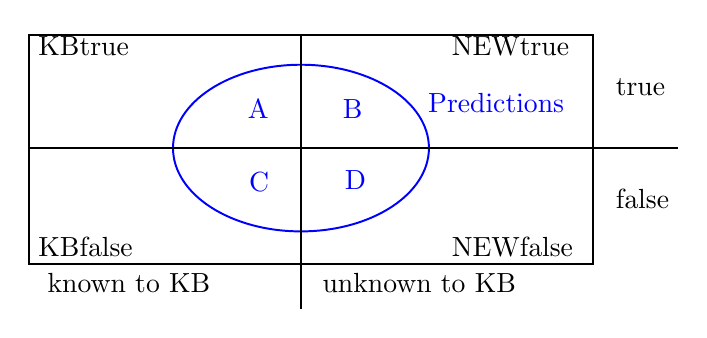
\begin{tikzpicture}

% Fabian: Keep figure in two colors.
% Even if printed in black and white, it's still clear enough

  \path[draw=blue, line width=0.7086614168764338] (3.708333, -1.458333) ellipse (1.625000 and 1.058333);
  \node[above, right, color=blue, font=] at (5.2000, -0.88333) {Predictions};
  \node[above, right, color=blue, font=] at (2.908333, -0.958333) {A};
  \node[above, right, color=blue, font=] at (4.116667, -0.966667) {B};
  \node[above, right, color=blue, font=] at (2.925000, -1.891667) {C};
  \node[above, right, color=blue, font=] at (4.141667, -1.866667) {D};
  \node[above, right, color=black, font=] at (0.250000, -0.166667) {KBtrue};
  \node[above, right, color=black, font=] at (0.250000, -2.708333) {KBfalse};
  \node[above, right, color=black, font=] at (5.500000, -0.166667) {NEWtrue};
  \node[above, right, color=black, font=] at (5.500000, -2.708333) {NEWfalse};
  \node[above, right, color=black, font=] at (7.583333, -0.683333) {true};
  \node[above, right, color=black, font=] at (7.583333, -2.100000) {false};
  \node[above, right, color=black, font=] at (0.366667, -3.166667) {known to KB};
  \node[above, right, color=black, font=] at (3.858333, -3.166667) {unknown to KB};
  \path[draw=black, line width=0.7086614168764338] (0.250000, -0.016667) rectangle (7.416667, -2.933333);
  \draw[draw=black, line width=0.7086614168764338] (0.250000, -1.458333) -- (8.500000, -1.458333);
  \draw[draw=black, line width=0.7086614168764338] (3.708333, -0.025000) -- (3.708333, -3.500000);
\end{tikzpicture}

\label{fig:prediction}
\end{figure}

Our goal is to find rules that make true predictions that go beyond the current KB.
In Figure~\ref{fig:prediction}, we wish to maximize the area B and to minimize the area D.
There are two obvious challenges in this context: First, the areas NEWtrue and NEWfalse are unknown.
So if we wish to maximize B at the expense of D, we are operating in an area outside our KB.
We would want to use the areas KBtrue and KBfalse to estimate the unknown area.
This, however, leads to the second challenge: Semantic KBs do not contain negative evidence.
Thus, the area KBfalse is empty.
This is the central challenge of our setting: to provide counterexamples for the rule mining.
These can take the role of KBfalse so that we can estimate the areas NEWtrue and NEWfalse.
We describe two approaches to this problem:
Creating counterexamples according to the Closed World Assumption (CWA) that traditional association rule mining systems apply and according to the Partial Completeness Assumption (PCA) that we propose.
We will now present these approaches in detail.
% There are several approaches to this problem:
% The standard confidence, the standard positive-only learning evaluation score of ILP, and the partial completeness assumption that we propose.
% We will now present these approaches in detail.



\subsection{The CWA and Standard Confidence} \label{subsubsec:stdConf}
The standard confidence measure takes all facts that are not in the KB (i.e., NEWtrue and NEWfalse) as negative evidence.
Thus, the standard confidence of a rule is the ratio of its predictions that are in the KB, i.e., the share of A (KBtrue)
in the set of predictions:

\[conf(\vec{B} \Rightarrow r(x,y)) := \frac{supp(\vec{B} \Rightarrow r(x,y))}{\#(x,y): \exists z_1,...,z_m: \vec{B}}\]\\

\noindent For example, consider again the rule
\indented{
$R:livesIn(x,y)\Rightarrow wasBornIn(x,y)$}
together with the KB given in Table~\ref{tab:exampleKB}. In this case, $conf(R)=1/3$, because (a) there is one positive example for the rule, $wasBornIn(Adam, Paris)$, and (b) the predictions $wasBornIn(Adam, Rome)$ and $wasBorn(Bob,Zurich)$ are counted as negative examples since they do not appear in the KB.

Standard confidence is the measure traditionally used in association rule mining and market basket analysis, where the Closed World Assumption (CWA) is used:
if there is no evidence in any of the transactions of the database that a user bought a specific product, then this user did not buy the product.
Albeit natural for the market basket analysis scenario, standard confidence fails to distinguish between ``false'' and ``unknown'' facts,
which makes it inappropriate for a scenario with Open World semantics like ours. Moreover, we also pursue a different goal than market basket analysis:
we aim to maximize the number of true predictions that go beyond the current knowledge,
whereas market basket analysis usually tries to mine rules that can describe data that is already known.






\ignore{
\subsection{Positives-Only Learning}
For cases where the KB does not contain negative examples, Muggleton has developed a \emph{positives-only evaluation score} for ILP \cite{Muggleton:1996:LPD:647996.742465,usir1753}.
It takes random facts as negative evidence:
\[ Score := log(P)-log\frac{R+1}{Rsize+2}-\frac{L}{P} \]
Here, $P$ is the number of known true facts covered (KBtrue, or A resp., in Figure~\ref{fig:prediction}), $R$ is the number of random examples covered, $Rsize$ is the total number of randoms, and $L$ is the number of atoms in the hypotheses. \comment{Katja}{is ``randoms'' a well-defined term?}
The intuition is that a good rule should cover many positive examples, and few or no randomly generated examples. This ensures
that the rule is not overly general. Furthermore, the rule should use as few atoms as possible, and thus achieve a high compression.
This measure is implemented (among others) in the ALEPH system.

% \comment{Fabian}{Give intuitive reason why this measure is not good, to justify our own measure. Check:}
% The disadvantage of this measure is that it ``guesses'' negative examples at random.
% Even if a rule produces many false predictions, the intersection of these false predictions and the random counterexamples may be very small.
% In section~\ref{sec:experiments}, we compare ALEPH with our method.


%\comment{Fabian}{Give intuitive reason why this measure is not good, to justify our own measure.}
%\comment{Chris}{I gave it a try. Please have a look.} % Looks good, thanks!
% \comment{Fabian}{Thanks for the explications, Christina! Can we have a rule that is intuitively false? I tried to change the example, please modify if wrong.}

The disadvantage of this measure is that it ``guesses'' negative examples at random, whereas rules usually create false predictions in a non-random way.
Even if a rule produces many false predictions, the intersection of these false predictions and the random counterexamples may be very small.
Consider for example the rule $bornIn(x,y) \Rightarrow diedIn(x,y)$, which produces false predictions for example for persons who have moved
to a different place during their life.
By creating negative examples just by considering random person-location pairs,
we might not produce any case for which the rule will give a false prediction, % (person re-married with someone's mother),
simply because such a negative example will have a relatively small probability to be generated.
In section~\ref{sec:experiments}, we compare this measure to our method, which we introduce next.
}


\subsection{The PCA and the PCA-Confidence}\label{subsubsec:pcaConf}

In AMIE, we generate negative examples for a rule by means of the \emph{Partial Completeness Assumption} (PCA).
The PCA is the assumption that if $r(x,y) \in$ \emph{KBtrue} for some $x,y$, then
\begin{multline*}
\forall y': r(x,y') \in \mbox{\emph{KBtrue}}\ \cup\ \mbox{\emph{NEWtrue}} \\\Rightarrow r(x,y') \in \mbox{\emph{KBtrue}}
\end{multline*}
In other words, we assume that if we know one $y$ for a given $x$ and $r$, then we know all $y$ for that $x$ and $r$.
This assumption allow us to generate counter-examples in a way that is less restrictive than the standard confidence.
In our example from Table~\ref{tab:exampleKB}, the PCA will assume that any other place of birth for
Adam and Carl is false. Conversely, the PCA will not assume anything about the places of birth of Bob, because
the KB does not know any.
With this notion in mind, we redefine the definition of confidence for rules. Under the PCA,
the denominator of the confidence formula is not the size of the entire set of conclusions
derived from the body of the rule,
but the number of facts that we know to be true together with the facts that we assume to be false.

\begin{small}
\begin{multline} \label{eq:pcaConf}
 \hspace*{-2ex}
conf_{pca}(\vec{B} \Rightarrow r(x,y)) :=\\ \frac{supp(\vec{B} \Rightarrow r(x,y))}{\#(x,y): \exists z_1,...,z_m,y': \vec{B} \wedge r(x,y')}
\end{multline}
\end{small}
%
This formula normalizes the support by the number of pairs $(x,y)$ for which there exists a $y'$ with $r(x,y')$.
Consider again the KB given in Table~\ref{tab:exampleKB} and the rule $R: livesIn(x,y)\Rightarrow wasBornIn(x,y)$. In this case, $conf_{pca}(R)=1/2$. This is because (a) there is one positive example for the rule, $wasBornIn(Adam, Paris)$, and (b) the prediction $wasBornIn(Adam, Rome)$ is counted as negative example, because we already know a different place of birth for Adam. The prediction $wasBorn(Bob,Zurich)$ is completely disregarded as evidence, because we neither know where Bob was born nor where he was not born.

Notice that Eq.~\ref{eq:pcaConf} fixes $x$ and $r$ and implies that rules will try to predict values for $y$.
AMIE always predicts in the most functional direction. To see this, recall that
it is more intuitive to predict the birthplace of a specific person
than predict all the people that were born in a specific city.
Since in Sec.~\ref{subsec:functions} we re-write all relations so that their functionality
is larger than their inverse functionality, the most functional direction
will be always to predict $y$ given $x$.

In spite of being an assumption, the PCA is certainly true for functions, such as \emph{birthdate} and \emph{capital}.
The PCA also holds for relations that are not functions but that have a high functionality,
as we shall see in our qualitative analysis of the PCA in Section~\ref{experimentspca}.
The PCA has been applied in the Google Knowledge Vault under the name ``local completeness assumption'' \cite{knowledgevault}.






 %%%%%%%%%%%%%%%%%%%%%%%%%%%%%%%%%%%%%%%%%%%%%%%%%%%%%%%%%%%%%%%%%%%%%%%%%%%%%%%%%%%%%%%%%%%%%%%%%%%%

 % previous version from here


% \subsubsection{Qualitative Evaluation of the PCA}
% \label{pcaEvaluation}
%
% Since the PCA is one of the basic ingredients of AMIE,
% we wanted to know whether the PCA holds for a real world KB.
% For this purpose, we looked into each of the 33 relations between entities in YAGO2.
% For each relation $r$, we randomly sampled 30 subjects.
% For each subject $x$, we checked whether the KB knows all $y$ with $r(x,y)$.
% As a ground truth, we took the Wikipedia page of $x$ and what we could find on the Web by a search engine.
% It is obvious that such an evaluation cannot be done strictly quantitatively.
% For example, a person might have worked for a company, but this fact might appear nowhere on Wikipedia -- or even on the Web.
% Or a musician might play 10 instruments at different levels of proficiency, but Wikipedia mentions only the 4 main instruments.
% Even a search on the Web might not tell us that there are more than 4 instruments.
% Therefore, we resorted to a qualitative analysis.
% We analyzed each of the relations manually, and grouped the relations into categories.
% Some relations fall into multiple categories. \ignore{We also compare the PCA to the closed world assumption (CWA), i.e., the assumption that all facts that are not in the KB are false. This is the assumption on which the standard confidence measure relies.}
% % \comment{Fabian}{Could you check whether the relations you evaluated are placed right? (See spreadsheet) The relations with a question mark need additional checking...}
% %For this purpose, we randomly chose 30 entities and checked if there are missing facts about each entity-relation pair using the whole Web and common sense as ground truth.
% % Driven by these initial results that focused on answering the question whether the PCA holds for an average fact that is assumed to be false,
% % we also analyzed qualitatively whether the PCA holds for a particular entity-relation combination.
% % For this purpose, we randomly chose 30 entity-relation pairs and examined whether the assumption holds or not using the whole Web and common sense as ground truth.
% %\comment{Katja}{Is that true?}
% Table~\ref{PCA_assumption_entities} summarizes our findings.
% % by proposing a categorization of the problems we encountered and relating them to example relations that fall into these categories.
%
% % \ffigure{Table}{PCA_assumption_entities}{Categories of relations w.r.t. the PCA}{
% % \begin{tabular}{p{2cm}|p{5.4cm}}
% % \centering{Category}		  & Relations 	\\
% % \hline
% % Functions   & \emph{wasBornIn}, \emph{diedIn}, \emph{hasCapital}, \emph{hasCurrency*}, \emph{happenedIn}, \emph{hasPredecessor*}, \emph{owns}$^{-1}$ \\
% % Quasi-Functions & \emph{hasOfficialLanguage}, \emph{graduatedFrom}, \emph{isCitizenOf}, \emph{directed}$^{-1}$, \emph{hasAcademicAdvisor}, \emph{created}$^{-1}$, \emph{isLeaderOf}, \emph{wroteMusicFor?}$^{-1}$\\
% % \hline
% % Granularity Differences& 	$isLocatedIn$, \emph{happenedIn?}\\
% % \hline
% % Time Agnosticism \ignore{and implicit assumptions Fabian: What is this?} & $livesIn$, $worksAt$, $isCitizenOf?$, \emph{hasCapital?}, \emph{isMarriedTo}\\
% % % Implicit assumptions & $livesIn$, $isCitizenOf$\\
% % %Knowledge representation & $isMarriedTo$, $hasChild$, $actedIn$, $playsFor$, $worksAt$, $isPoliticianOf$\\
% % Extraction Incompleteness& \emph{participatedIn}$^{-1}$, \emph{produced}$^{-1}$,  \emph{actedIn}$^{-1}$, \emph{playsFor}, \emph{holdsPoliticalPosition}, \emph{hasChild}$^{-1}$, \emph{graduatedFrom}, \emph{hasWonPrize}, \emph{dealsWith}\\
% % %$influences$, $dealsWith$, $participatedIn$, $hasMusicalRole$, $livesIn$, $holdsPoliticalPosition$, $hasWonPrize$, $imports$, $exports$\\
% % Source Incompleteness & \emph{influences}$^{-1}$, \emph{imports}, \emph{livesIn}, \emph{holdsPoliticalPosition}, \emph{worksAt}, \emph{hasMusicalRole}, \emph{dealsWith}, \emph{isInterestedIn}, \emph{isKnownFor}
% % \end{tabular}
% % }
%
%
%
% \paragraph{Functions} YAGO2 contains several functions. For these, the PCA holds by definition.
% The PCA extends to relations that are not strictly speaking functions, but that have a high functionality.
% These are relations that usually have one object per subject, even though there could be multiple.
% For example, a person can graduate from several universities, but most people graduate from a single university.
% In all of these cases, the PCA worked very well, and predicted completeness correctly for $73\%-100\%$ of the subjects under investigation.
% Thanks to the FUN-property, the PCA also holds for quasi inverse-functional relations such as \emph{directed}.\\
%
%
% \ffigure{Table}{PCA_assumption_entities}{Categories of relations w.r.t. the PCA}{
% \begin{tabular}{p{2cm}|p{5.4cm}}
% \centering{Category}		  & Relations 	\\
% \hline
% Functions   & \emph{wasBornIn}, \emph{diedIn}, \emph{hasCapital}\\%,  \comment{Chris}{have we evaluated those guys?} \comment{Luis: }{These relations do not exist in YAGO2, only in YAGO2s} \emph{happenedIn}, \emph{hasPredecessor}, \emph{owns}$^{-1}$ \\
% \hline
% Quasi-Functions & \emph{hasCurrency}, \emph{hasOfficialLanguage}, \emph{graduatedFrom}, \emph{isCitizenOf}, \emph{directed}$^{-1}$, \emph{hasAcademicAdvisor}, \emph{created}$^{-1}$,  \emph{isLeaderOf}, \emph{isPoliticianOf}, \emph{isAffiliatedTo}\\%, \comment{Chris}{have we evaluated those guys?} \emph{wroteMusicFor}$^{-1}$\\
% \hline
% Granularity Differences& 	\emph{isLocatedIn},  \emph{livesIn}\\%,\comment{Chris}{have we evaluated those guys?} \emph{happenedIn}\\
% \hline
% Implicit Assumptions&\emph{livesIn} \\
% \hline
% Source Incompleteness & \emph{influences}$^{-1}$, \emph{imports}, \emph{exports}, \emph{actedIn}$^{-1}$, \emph{worksAt}, \emph{hasMusicalRole}, \emph{dealsWith}, \emph{isInterestedIn}$^{-1}$, \emph{isKnownFor}$^{-1}$\\
% \hline
% Extraction Incompleteness& \emph{participatedIn}$^{-1}$, \emph{isMarriedTo}, \emph{produced}$^{-1}$,  \emph{actedIn}$^{-1}$, \emph{playsFor}, \emph{holdsPoliticalPosition}, \emph{hasChild}$^{-1}$,  \emph{hasWonPrize}, \emph{dealsWith},\emph{influences}$^{-1}$, \emph{hasMusicalRole} \\
% \end{tabular}
% }
%
% \paragraph{Granularity Differences} Some relations, such as \emph{locatedIn} and \emph{livesIn}, hold between an entity and a geographical region.
% In that case, the region can be given at the granularity of a city, a region, a country, or a continent.
% Naturally, if YAGO contains one of these, the others are possible options, and thus the PCA does not hold.
% However, these cases could be addressed if one restricts the range of the relation.
% With such a restriction, the relations become functions or quasi-functions, which lifts them into the category where the PCA works well.
% We plan to investigate this possibility in future work.
%
% % \paragraph{Time Agnosticism} \comment{Chris}{I suggest to erase the time agnosticity.
% % What I meant back then is that the infobox might contain as residence only the last residence (and therefore YAGO knows only that one),
% %  but we take as correct all residences. I assume that we can consider this as a case of incomplete extraction.}
% % \comment{Fabian}{I think it makes an interesting special case, also with marriedTo}
% % For some relations, the KB is time agnostic: It contains only one object for a given subject, even though other objects may have held at other points of time.
% % For example, a person might have lived in many different places during her life and all the corresponding facts are considered to be true.
% % However, the KB might contain only the latest of these facts.
%
%
% \paragraph{Implicit Assumptions} Some statements can be inferred from the Wikipedia page even if the page does not mention them. % For instance, %\emph{livesIn} is incomplete ``in-purpose'' in the sense
% People do not usually state information that can easily be inferred by what they have stated before
% (following Grice's Maxim of quantity and manner~\cite{grice}). %\footnote{\url{http://www.usingenglish.com/articles/grices-conversational-maxims.html}}).
% For example, if someone graduated from a university, people usually do not feel obliged to mention that this person used to live in the country,
%  in which the university is located,
% because this can easily be inferred by the reader. Only less obvious residences will be explicitly mentioned and therefore, PCA assumption will not hold.
% Note that rules such as $graduatedFrom(x,y)\Rightarrow livesIn(x,y)$, to follow the previous example, can only be mined if Grice's maxims are occasionally violated by the authors of the articles.
% If the authors follow the maxims always, then such rules cannot be mined, because there are not even positive examples for which the rule holds (lack of support).
% In the case of YAGO, the only relation that we found in this category is \emph{livesIn}.
%
%
% \paragraph{Source Incompleteness} For many relations, the source itself (Wikipedia) is incomplete.
% Usually, these relations have, for each subject, some objects that are undisputed.
% For example, it is undisputed that Albert Einstein is interested in physics. However, these relations also have objects that are less important, disputed, or unknown.
% For example, Albert Einstein might also be interested in music (he played the violin), but maybe also in pancakes.
% These less prominent objects are a lot less likely to appear in Wikipedia, or indeed in any Web page.
% Even if they do, we can never be sure whether there is not still something else that Einstein was interested in.
% For these relations, the knowledge sources are often incomplete by nature.
% For example, not every single product that a country imports and exports is explicitly mentioned.
% Whether or not this poses a problem depends on the application.
% If ground truth is defined as what is universally true, then source incompleteness is a problem.
% If ground truth is the source of the KB (i.e., Wikipedia in this case), then source incompleteness is not an issue.
% \comment{Luis}{Does isMarriedTo fall in this category? What about non-prominent spouses (without Wikipedia article)? We would not extract the inverse statement in that case.}
% \comment{CHris}{This is the case of extraction incompleteness. Wikipedia usually is pretty precise for the spouses. So it is complete. The fact
% that yago does not extract spouses that do not have their own wikipedia pages is a problem with the extraction. Not an incompleteness
% problem}
%
%
% \paragraph{Extraction Incompleteness} For a large number of relations, the Wikipedia page contains more objects for a given subject than the KB.
% These are cases where the extraction process was incomplete.
% In the case of YAGO, this is due to a strong focus on accuracy,
% which causes the extraction to discard any extracted fact that cannot be type checked or linked to an entity.
% This class of relations is the most sensitive category for the PCA.
% The success of the PCA will depend on how many relations and to what extent they are affected by incomplete extractions.
% \comment{Chris}{Do we have precision numbers for this category?}
% % Furthermore, there are relations which are sometimes open to subjective interpretation.
% % For example, it is difficult to decide whether a particular person was actually influenced by another person that he or she met.
%
% \paragraph{Discussion} In summary, our analysis shows that it depends on the nature of the relation and on its type signature whether the PCA holds or not.
%  There are a large number of relations for which the PCA is reasonable.
% These are not just functions and inverse functions, but also relations that exhibit a similar behavior.
%
% For many other cases, the PCA does not hold. In these cases, AMIE will wrongly assume that a rule is making incorrect predictions -- although, in reality,
% the predictions might be correct.
% Thus, when the PCA does not hold, AMIE will err on the side of caution.
%
% At the same time, the PCA is not as restrictive as the closed world assumption (CWA):
% PCA admits that there can be facts that are true, but not known to the KB.
% \ignore{If we compare the PCA to the CWA, we note that the CWA assumes that all facts that are not in the KB are false. Consider a function $r$ and an entity $x$. If there exists an $y$ with $r(x,y)$ in the KB, then the CWA holds: Any fact of the form $r(x,y')$ with $y'\neq y$ is false. However, if there is no $y$ with $r(x,y)$, then the CWA does not hold. The CWA would wrongly assume that there cannot be a $y$ with $r(x,y)$. } For example, if a person has a birth date, then both CWA and PCA would not admit another birth date. However, if a person does not have a birth date, then the PCA will admit that there can be a birth date, while the CWA will assume that there cannot be a birth date. Thus, the PCA is more permissive than the CWA.
% This encourages us to use the PCA for the definition of our confidence. In our experiments, we will show that this definition of confidence produces
%  more predictive and more accurate rules than the standard confidence, which is based on the CWA.
%

 % previous version until here
 %%%%%%%%%%%%%%%%%%%%%%%%%%%%%%%%%%%%%%%%%%%%%%%%%%%%%%%%%%%%%%%%%%%%%%%%%%%%%%%%%%%%%%%%%%%%%%%%%%%%

%We will evaluate the PCA in the context of rule mining next.


% \comment{Fabian}{Old text follows. I tried to subsume it in the classification above. I would propose to remove what follows, for the reasons given below:}
%
%
% % PCA might be a reasonable assumption or not, depending on the nature of the head relation and its type signature.
% For example, for relations with strong functional or inverse functional behavior, such as $diedIn$ and $directed$,
% PCA successfully predicts negative facts (ratio=100\% in Table~\ref{PCA_assumption_rules}).
% On the other hand, $livesIn$ is a relation for which PCA does not hold.
% The reason for this is manifold; and results from both the type signature of $livesIn$ and its nature. For example, consider the rule $isCitizenOf(x,y) \rightarrow livesIn(x,y)$.
% If the KB contains the information in which city a specific person lives and the rule predicts the corresponding country, then the predicted fact is counted as negative although it is not because the city is located in the predicted country. This is also true for the relation $isLocatedIn$.
% In other words, PCA is sensitive to predictions that contain arguments involved in a strict functional hierarchical relation that expresses granularity, e.g., a particular city is in general located in a particular region, a region in a country, and so on.
% %A possible solution to counteract this problem is to consider the type system as well as the domain/range information that is provided by the KB. The approach proposed in this paper, however, still ignores such information but we plan to integrate this aspect in our future work.
% % In other words, PCA is sensitive to granularity effects that might exist between the different relations.
% % However, this issue might be tackled if in the future we make use of the type system and domain/range information of the KB, which for the time being we ignore.
%
% There is another problem category that the $livesIn$ relation falls into:
%
% \ignore{
% \comment{Chris}{Do we actually need the following one? I think it does not fit in this context. Perhaps move it to the model section?}
% \comment{Fabian}{I wrote it, but I think it should just be removed, unless someone protests}
% On the other hand, according to Grice's conversation maxims we should not say something that can lead to false conclusions.
% I.e., if someone states that Priscilla Presley has a child (which is not false but incomplete as she actually has two children),
% humans would infer that she has only one child and this is also how the PCA assumption would interpret the information.
% % On the other hand, if someone states that Priscilla Presley has one child, then this is not false but incomplete as she actually has two children.
% % However, humans would understand that she has not more than one child and this is also how the PCA assumption would interpret the information.
% %\comment{Fabian}{Interesting! Grice's maxim can also be used to explain why the PCA makes sense. Look at Priscilla. She has 2 children. If we say "Priscilla has 1 child", that is not false. But it is not complete. Thereby, we violate Grice's maxim.}
% This phenomenon makes information extraction very difficult and results in PCA being less accurate for some relations.
% }
% $worksAt$ and $isCitizenOf$ are additional examples of relations that are both time agnostic and often go along with implicit assumptions. \comment{Katja}{Split up into two categories?}
% In general, this group of relations is very difficult to capture because of the lack of information that can be exploited by machines
% and because it eventually requires to understand how the human brain works.
% But nevertheless, AMIE is able to mine such rules even though the predicted precision does not always exactly match the actual precision. \comment{Fabian}{Here, we do not yet talk of rules, do we?}
%
% We also noticed that for relations for which functionality and inverse functionality (Section~\ref{subsec:functions}) have similar values
% (e.g., $isMarriedTo$, $hasChild$), PCA might also show some deficiencies.
% For such relations it is not clear which variable is the input and which one is the output (e.g., parent or child, husband or wife).
% \comment{Fabian}{From the theoretical point of view, this is not a problem: If the KB contains people that have many children, then hasChild is de facto inverse functional, in China it is de facto functional.}
% In cases in which it is not clear if the fact relates more with the subject or the object we observe the following problem:
% the information about these relations is often scattered on Wikipedia pages of both entities in the relation,
% e.g., two persons might get married and only one of the Wikipedia pages is updated. \comment{Fabian}{We should not argue this way, because it basically means that we were too lazy to extract the information manually from Wikipedia. We could have manually scanned the download of Wikipedia (the XML dump) for the spouse, and we would have found him/her.}
% We have also found these problems to be true for several N:M relations such as $actedIn$ and $playsFor$.
% In summary, the problems that occur with these relations originate from the knowledge representation both in the KB
% as well as in the knowledge source, in our case Wikipedia.
% Since for these relations it is not clear which variable is input and which output, a possible solution that we plan to consider
% in our future work could be to mine two versions of a rule.
% For example when learning the relation $actedIn$, once actor is the input and movie the output and once the other way round.
%
% % Another source of problems are extraction failures, i.e., during the construction of the KB by extracting information from sources such as Wikipedia the content is misunderstood,
% %  which results in false facts in the KB. This is especially true for relations that are difficult to extract in general such as $dealsWith$ and $influences$.
% % \comment{Fabian}{Do we have really false extractions? Or only incomplete extractions? If we do, that would be an additional category}
% % As AMIE so far relies on the input contained in the KB and assumes facts in the KB to be true, this naturally leads to problems during rule mining.
%
% A possible solution would be to combine rule mining and knowledge extraction and use mutual feedback:
% the rule mining part can create "possibly true`` facts and then an information extraction component will try to extract exactly those facts from the source.
% If new facts can be added to the KB from the information extraction component, new rules can potentially be learned by the rule mining component.
% \comment{Fabian}{I love this idea! The problem is that the incompleteness kills the PCA, and thus AMIE will exactly not mine the ``expected'' rules and facts, no? It seems that we are shooting ourselves in the knee here...}

% \comment{Chris}{move to experiments or completely off}
%
% \subsection{PCA in Rule Mining}
% %\comment{Chris}{I moved it as a paragraph under the quality evaluation, because I think it logically belongs here. You can move it around if you wish.}
% We have seen that the PCA holds for some relations, but is too optimistic about the completeness of the KB for many others.
% We wanted to evaluate how this influences the rule mining in AMIE.
% Whenever AMIE mines a rule $\vec{B} \Rightarrow r(x,y)$, she will look at all facts that the rule can predict.
% Conceptually, AMIE will group the predictions into three categories:
% Either the prediction appears in the KB, then it is a positive example.
% The prediction can also be rejected by the PCA, and then it is a negative example.
% Finally, the prediction can be neither a positive example nor a negative example, but just an statement of unknown truth.
% Now, we are interested in the negative examples.
% These fall again into two categories: True negative examples ($TN$)  are statements that are false in reality ($TN \subseteq NEWfalse$).
% False negative examples ($FN$) are statements that were assumed to be false, but are true in reality ($FN \subseteq NEWtrue$).
% We want to measure how often the assumed negative examples were indeed negative examples.
% For this reason, we ran AMIE on YAGO\footnote{We used the version ``YAGO2''} and collected the resulting rules.
% For each rule, we sampled 30 predictions that the PCA called false negative examples.
% \comment{Fabian}{Did we do that for all rules? Or only for the rules with a high PCA confidence? If we did the latter, then we are not being fair, no?}.
% \comment{Chris}{It is only for the top 30 in PCA. }
% We manually evaluated them, using Wikipedia as ground truth.
% For each head predicate, we report the average of  $\frac{|TN|}{|TN+FN|}$ among all rules with this specific head,
% weighted by the total number of assumed negatives for each rule (micro-average).
% We call this measure $precOnNeg$:
%
% \[
%  precOnNeg(r_h)=\frac{\sum \limits_{all \; R \; with\; r_h \;in \; head }{ |TN(R)|}}{\sum \limits_{all \; R \; with\; r_h \;in \; head }{|TN(R)+FN(R)|} }
% \]
%
% The results are shown in Table~\ref{PCA_assumption_rules}.
% Our results show that the PCA works very well in practice:
% In the vast majority of cases where the PCA rejects a prediction, that prediction is indeed wrong.
% This is trivially true for functional relations such as \emph{diedIn}, but holds also for many other relations.
% \emph{livesIn} is a particularly hard case: It suffers from granularity differences and implicit assumptions.
% Hence, the PCA does not work well for this relation.
%
%  \ffigure{Table}{PCA_assumption_rules}{Ratio of facts correctly assumed to be false}{
% \begin{tabular}{l|c}
% %head predicate		  & $TN/(TN+FN)$ \% 	\\
% \textbf{Head Predicate} & $precOnNeg$ \% 	\\
% \hline
%   $created$		&86.67	\\
%   $diedIn$		&100	\\
%   $directed$		&100 	\\
%   $hasChild$		&60.74	\\
%   $hasOfficialLanguage$	&75	\\
%   $isCitizenOf$		&80.03	\\
%   $isLeaderOf$		&90	\\
%   $isMarriedTo$		&83.82	\\
%   $isPoliticianOf$	&73.15	\\
%   $livesIn$		&7.75	\\
%   $produced$		&93.87	\\
%   $worksAt$		&89.66	\\
% \end{tabular}
% }
% \comment{Fabian}{In the ideal case, we would compute the numbers for the CWA here and compare...}
%
% \paragraph{Discussion}
% %Note that despite these problems, % Fabian: There is no problem, PCA is great! :-)
% We see that the PCA performs well in general in the rule mining scenario.
% This is true in particular if we compare it to the alternative, the Closed World Assumption (CWA).
% The CWA would reject all statements that are not in the KB as false.
% This includes the statements that the PCA assumes to be false. Thus, there are cases in which both assumptions err.
% For example, if the KB contains only one parent of a child, then both assumptions would (erroneously) reject an additional parent.
% One way to mitigate this would be to learn an ``expected cardinality'' of a relation, and to reject as false everything that goes beyond this cardinality.
% This, however, would require coordination across rules if the number of objects in the KB falls more than 1 object short of the expected cardinality
% -- something that we defer to future work.
% \comment{Chris}{I didn't get it}
% In all other cases, the PCA is more accurate than the CWA:
% The CWA will not admit a birthplace for a person that does not have a birthplace in the KB. The PCA will.
% Likewise, the CWA will not admit parents for a child that does not have parents in the KB, while the PCA does.
% This shows that the PCA is more careful when producing negative examples. This will help AMIE mine more productive rules, as we shall see later.
% %Thus, even more facts are assumed to be false, i.e., all the facts that are not contained in the KB.
% %This set of facts consists of (i) facts assumed to be false under PCA and (ii) facts that normally exist for similar entities.
% %An error (FN) resulting from (i) could be that the KB contains, for example, only information about 1 out of 2 children ($childOf$). % Fabian: hasChild is inverse functional, the argument would have to be turned around.
% %For this case, both CWA and PCA would draw the wrong conclusion.
% %However, an error (FN) resulting from (ii) occurs if the KB, for example, does not contain a birthdate for a particular person;
% %under CWA, this means that the person has no birthdate whereas under PCA, this means that the fact is unknown.
%
